\section{Introduction}

In computing systems, performance and energy consumption are conflicting goals -- increasing performance requires a super-linear increase in power consumption.
As power and energy become first-class concerns in systems ranging from low-power embedded platforms to large scale high-performance computing (HPC) environments, there is an increasing need for software to manage hardware resource allocations to achieve a desirable balance in performance and power/energy consumption.
Fortunately, modern systems expose knobs to support trading performance and power.
For example, dynamic voltage and frequency scaling (DVFS) trades processor clock rate and power consumption for changes in throughput, and is ubiquitous in modern systems.
Another common approach is to change the allocation of compute cores on multicore systems, allowing unallocated cores to enter low-power sleep states, or even shut down altogether to save power/energy.

Thermal design constraints limit both the maximum and average performance that a computing system can achieve.
To understand the behavior of a particular application on a system, we can perform a characterization by testing it in each system configuration and recording the behavior.
Performance and power typically form a non-linear, convex tradeoff space, where each system configuration, \eg DVFS setting, produces unique application performance and system power values.
% \TODO{Show an example.}

However, heuristic approaches to balancing performance and power/energy rely on assumptions about the performance/power tradeoff space of an application and system that we have found are not portable between applications and systems (as we demonstrated on embedded platforms in \cite{Imes2014}).
For example, the classic race-to-idle heuristic can achieve low energy consumption on one system, but high energy consumption on another compared with a pace-to-idle or never-idle approach.
An important observation by Kim \etal is, ``Unless the function of a given machine is a straight line originating from the idle state, (0, $P_{idle}$), an idling heuristic is never optimal for all instances'' \cite{kim-cpsna2015}.
In short, the more convex the tradeoff space, the further from optimal any idling approach is.

\begin{figure}[t]
  \begin{centering}
  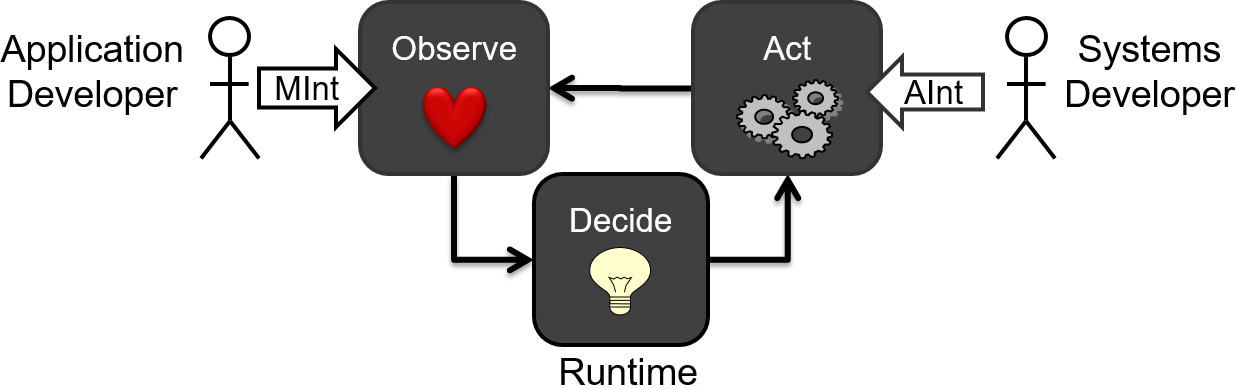
\includegraphics[width=0.6\textwidth]{figs/SEEC.png}
  \caption{A self-aware computing (SEEC) runtime model -- observe, decide, and act.}
  \label{fig:seec}
  \end{centering}
\end{figure}

The lack of both portability and optimality of heuristics demand that we develop more general approaches to addressing the problems in balancing performance and power.
In his PhD thesis, Hoffmann proposes a ``self-aware'' computing model (SEEC) that uses a closed-loop feedback design to \emph{observe}, \emph{decide}, and \emph{act} \cite{HoffmannPhD}.
\figref{seec} demonstrates this concept.
The SEEC model is more portable than many heuristics because it includes an observation step that measures behavior at runtime rather than relying strictly on assumptions made offline.
We build on this high-level model and use feedback systems that measure application and system behavior during runtime to make changes to resource allocations as new information becomes available.
Furthermore, our general feedback system designs do not depend on extremely accurate or complete models -- they instead rely on runtime measurements to fine-tune their decisions.

This thesis addresses two common goals in managing performance and power consumption.
The first is meeting an application performance goal while minimizing the total energy consumption.
We formulate this as a constrained optimization problem, using control theory to meet the performance goal, and linear optimization to select the optimal pair of system configurations to use that satisfy the performance constraint.
This approach is practical since in the aforementioned work, Kim \etal prove that an optimal solution to this constrained optimization problem requires, at most, two system configurations from the convex hull of the tradeoff space \cite{kim-cpsna2015}.
The second approach addresses the problem of running software as energy-efficiently as possible, \ie maximizing the ratio of work completed to energy consumed.
We treat this as a classification problem, using samples from low-level hardware performance counters to drive well-understood machine learning approaches that predict the most energy-efficient configuration to use.
This approach does not require the software to provide its own instrumentation, nor does the classifier need to know anything about the application in advance.
